% !TeX spellcheck = es_ES
\documentclass[12pt, titlepage]{article}
\usepackage[utf8]{inputenc}
\usepackage[spanish]{babel}
\usepackage{float}
\usepackage[letterpaper, margin=2.5cm]{geometry}
\usepackage[nottoc,notlot,notlof]{tocbibind} % Hace que se agregen las referencias al indice
\usepackage{url}
\usepackage{graphicx} 
\usepackage{listings}
\usepackage{color}
\definecolor{dkgreen}{rgb}{0,0.6,0}
\definecolor{gray}{rgb}{0.5,0.5,0.5}
\definecolor{mauve}{RGB}{253,151,31}

\lstset{frame=tb,
    language=Sql,
    aboveskip=3mm,
    belowskip=3mm,
    showstringspaces=false,
    columns=flexible,
    basicstyle={\small\ttfamily},
    numbers=none,
    numberstyle=\tiny\color{gray},
    keywordstyle=\color{blue},
    commentstyle=\color{dkgreen},
    stringstyle=\color{mauve},
    breaklines=true,
    breakatwhitespace=true,
    tabsize=2,
    morekeywords={use}
}

\title{Tarea 3: Índices}
\author{Carlos Tonatihu Barrera Pérez \\ Profesor: Hernández Contreras Euler \\ Bases de Datos \\ Grupo: 2CM1 }
\date{31 de marzo de 2017}

\begin{document}
	\maketitle
	\tableofcontents
	\section{Introducción}
	Los Índices surgen debido a que al hacer muchas consultas estas pueden hacer referencia a una pequeña porción de los registros de un archivo por lo que se genera un gasto adicional en la búsqueda de estos registros por lo que al implementar índices esto se puede mejorar.
	
	Los índices en las bases de datos cumplen la misma función que el índice de un libro el cual es evitar búsquedas innecesarias para encontrar la información que se desea de la manera más rápida posible. 
	
	En este caso al recuperar algún registro con base en su identificador el sistema de bases de datos buscaría en un índice para encontrar el bloque de disco donde se ubica el registro correspondiente para después extraer el bloque y en seguida obtener el registro que se busca.\cite{LIBRO}
	
	Existen dos tipos de índices en la base de datos:
	\begin{itemize}
		\item \textbf{Índices ordenados}. Basados en una disposición ordenada de los valores.
		\item \textbf{Índices asociativos}. Basados en una distribución uniforme de los valores a través de cajones (buckets). El valor de cada cajón esta determinado por una función de asociación (hash función). 
	\end{itemize}
	No existe una técnica universal que se deba de utilizar sino que esto depende de la base de datos. Para realizar la eleccion indicada se debe de tomar en cuenta:
	\begin{itemize}
		\item Tipos de acceso
		\item Tiempos de acceso
		\item Tiempo de inserción
		\item Tiempo de borrado
		\item Espacio adicional requerido
	\end{itemize}
	\section{Desarrollo}
	\subsection{Primario}
	El indice primario es aquel en el cual el archivo que contiene los registros está ordenado secuencialmente y el indice cuya clave de búsqueda especifica el orden secuencial del archivo es el indice de agrupación (indice primario) ademas de que es un indice no denso. Índice primario hace alusión a un índice según la clave primaria aunque esto no es necesario.
	\begin{figure}[H]
		\begin{center}
			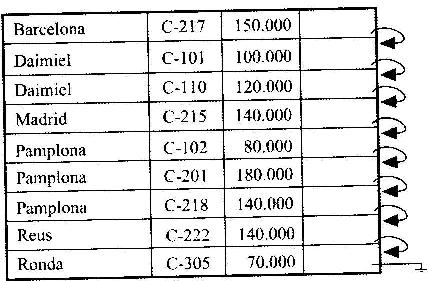
\includegraphics[width=10cm, height=5cm]{img/indiceprimario.jpg}
			\caption{Ejemplo de un indice primario ordenado secuencialmente con base en su clave.}
			\label{fig:hasta-use2}
		\end{center}
	\end{figure}
Este tipo de indices esta disponible en sistemas gestores de bases de datos como MySQL, SQLServer, PostgreSQL, Oracle y IBM DB2.
	\subsection{Secundario}
	El índice secundario es aquel en el que las claves de búsqueda especifican un orden diferente del orden secuencial del archivo.
	Este tipo de indice mejora el rendimiento de las consultas que utilizan otras claves de búsqueda distinta de la del indice primario.Sin embargo estos implican un gasto adicional en la modificación de la base de datos.
	\begin{figure}[H]
		\begin{center}
			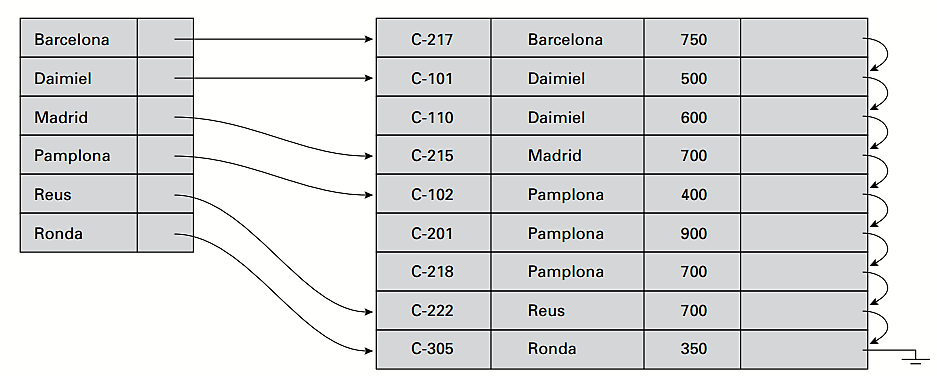
\includegraphics[width=14cm, height=5cm]{img/secundario.png}
			\caption{Indice secundario sobre el campo clave (denso).}
			\label{fig:hasta-use}
		\end{center}
	\end{figure}
En el caso de los indices secundarios sobre un campo no clave se tienen las siguientes opciones.
\begin{itemize}
	\item Existe una entrada por cada registro (indice denso).
	\item Registros de longitud variable. Indice no denso y el campo de la dirección contiene una lista de punteros.
	\item O registros de longitud fija. Indice no denso con un nivel extra de indirección para manejar punteros múltiples
\end{itemize}
	\begin{figure}[H]
	\begin{center}
		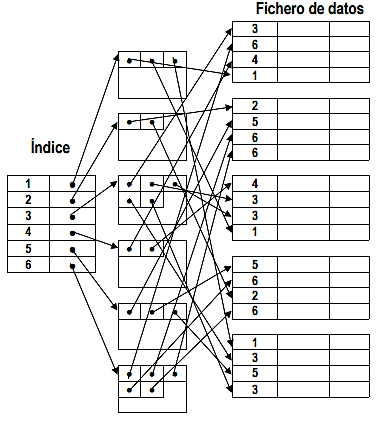
\includegraphics[width=8cm, height=8cm]{img/secundario2.png}
		\caption{Indice secundario sobre un campo no clave.}
		\label{fig:use}
	\end{center}
	\end{figure}
Este tipo de indices esta disponible en sistemas gestores de bases de datos como MySQL, PostgreSQL, Oracle y IBM DB2.
	\subsection{Agrupamiento}
	Un indice de agrupamiento es un índice no denso que tiene una entrada por cada valor distinto del campo de indexación.
	Sus entradas son registros de longitud fija, el campo de indexación que utilizan es un campo no clave de ordenación del fichero de datos, además, es un indice no denso. Es importante mencionar que en un fichero ordenado por un campo no clave solo se puede definir un indice de agrupamiento.
	\begin{figure}[H]
		\begin{center}
			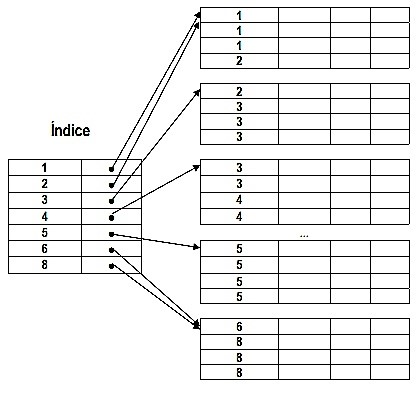
\includegraphics[width=8cm, height=8cm]{img/agrupamiento.jpg}
			\caption{Ejemplo de un indice de agrupamiento.}
			\label{fig:hasta}
		\end{center}
	\end{figure}
	Otro aspecto importante de este tipo de indices es que son registros de longitud fija en donde las entradas son una por cada valor distinto del campo de agrupamiento. Y el puntero apunta al primer bloque que contiene un registro con dicho valor.
	
	\subsection{Árbol $B^{+}$}
	Un indice de árbol $B^{+}$ tiene forma de un árbol equilibrado en el que cada camino de la raíz a las hojas tiene la misma longitud. Su altura es proporcional a el logaritmo base N del número de registros de la relación.
	
	Este tipo de árbol es más corto que los arboles binarios por lo que se necesitan menos accesos a disco para localizar los registros. Es por esto que las búsquedas son directas y eficientes pero al momento de realizar una inserción y borrado el trabajo se complica pero sigue manteniendo su eficiencia.
	
	Se utiliza para evitar el principal inconveniente de la organización del archivo secuencial indexado el cual es que el rendimiento disminuye conforme el archivo crece.
	
	\begin{figure}[H]
		\begin{center}
			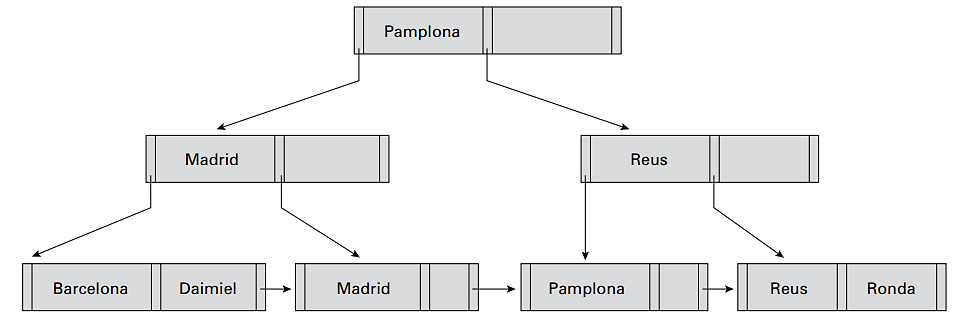
\includegraphics[width=16cm, height=5cm]{img/arbol.png}
			\caption{Estructura de un árbol n=3.}
			\label{fig:fd}
		\end{center}
	\end{figure}
En un nodo de este tipo se tiene que $K_{i}$ representa los valores de la clave de búsqueda y $P_{i}$ son los punteros a los hijos (si se trata de un simple nodo) o a los registros para los nodos hoja.
Como se puede observar en la figura \ref{fig:fd4} en un nodo las claves de búsqueda están ordenas de la forma $k_{1} < k_{2} < k_{3} < ... < k_{n-1}$.
\begin{figure}[H]
	\begin{center}
		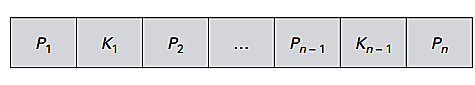
\includegraphics[width=14cm, height=2cm]{img/nodo.png}
		\caption{Estructura de un nodo del árbol n=3.}
		\label{fig:fd4}
	\end{center}
\end{figure}
Este tipo de indices esta disponible en sistemas gestores de bases de datos como MySQL, PostgreSQL, SQLServer, Oracle y IBM BD2.
\begin{figure}[H]
	\begin{center}
		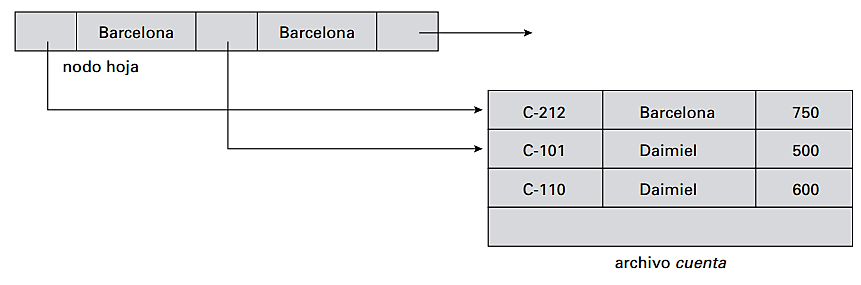
\includegraphics[width=16cm, height=5cm]{img/hoja.png}
		\caption{Ejemplo de un nodo hoja que apunta a un registro.}
		\label{fig:fd}
	\end{center}
\end{figure}
	
	\subsection{Múltiples niveles}
	El objetivo de los indices multinivel es reducir más que en la búsqueda binaria el fragmento de indice en donde se busca. Esto se realiza gracias a su estructura en donde el primer nivel es un fichero ordenado con entradas de tamaño fijo y un valor distinto del campo de indexación en cada una.
	
	En los siguientes niveles hay indices primarios sobre el primer nivel esto quiere decir que para un numero de registros por bloque $r$ en el primer bloque se tienen $i_{1}$ entradas, en el siguiente nivel hay $i_{2}= \frac{i_{1}}{r}$ entradas y en el tercer nivel $i_{3}= \frac{i_{2}}{r}$ por lo que se necesita un nivel más si el anterior ocupa más de un bloque.
	
	\begin{figure}[H]
		\begin{center}
			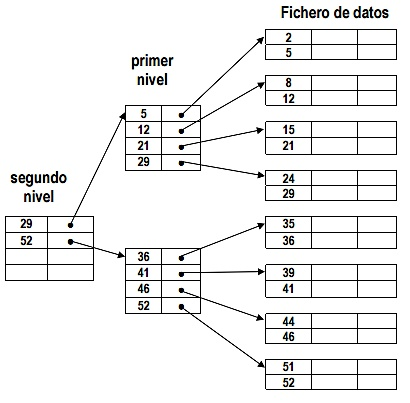
\includegraphics[width=8cm, height=8cm]{img/multinivel.jpg}
			\caption{Estructura de un índice multinivel de dos niveles.}
			\label{fig:mul}
		\end{center}
	\end{figure}
	\subsection{Tablas hash}
	Un índice de tabla hash consta de una colección de cubos organizados en una matriz. Además, una función hash asigna las claves de índice a los cubos correspondientes en el índice hash. Como se muestra en el ejemplo de la figura \ref{fig:hash} las tres claves de índice se asignan a tres cubos distintos en el índice hash. \cite{WEB}
	
	\begin{figure}[H]
		\begin{center}
			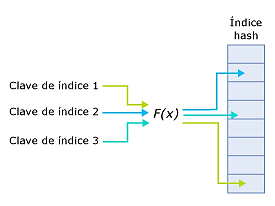
\includegraphics[width=7cm, height=6cm]{img/hash.png}
			\caption{Asignación mediante tabla hash.}
			\label{fig:hash}
		\end{center}
	\end{figure}
La función hash debe de tener las siguientes características:
\begin{itemize}
	\item La función hash es determinista. La misma clave de índice se asigna siempre al mismo cubo en el índice hash.
	\item Se pueden asignar múltiples claves de índice al mismo depósito de hash.
	\item La función hash está equilibrada, lo que significa que la distribución de los valores de clave de índice en los depósitos de hash sigue normalmente una distribución de Poisson
\end{itemize}
\begin{figure}[H]
	\begin{center}
		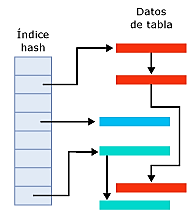
\includegraphics[width=6cm, height=6cm]{img/hash2.png}
		\caption{Tabla hash en memoria.}
		\label{fig:hash2}
	\end{center}
En memoria la estructura de índice hash consta de una matriz de punteros de memoria. Cada cubo asigna un desplazamiento en esta matriz. Cada cubo de la matriz señala a la primera fila del cubo de hash. Cada fila del cubo señala a la siguiente fila, por lo que genera una cadena de filas para cada cubo de hash como se observa en la figura \ref{fig:hash2}.

Este tipo de indices esta disponible en sistemas gestores de bases de datos como MySQL, PostgreSQL, SQL Server, Oracle y IBM BD2.
\end{figure}
	\section{Conclusiones}
	Este tema es bastante extenso por lo que se debe de conocer a fondo para elegir la técnica que mejores resultados nos brinde a la hora de implementar una base de datos, además de que se tiene que elegir la tecnología correcta para implementar dicha técnica.
	Además, se puede observar que la mayoría de este tipo de índices se puede utilizar en diversos sistemas gestores de bases de datos.
	Por ultimo, para algunas de estas técnicas considero que se requiere tener conocimientos de algoritmos y estructuras de datos para obtener resultados más óptimos y entender que esta sucediendo.
	\bibliography{bibliografia} 
	\bibliographystyle{ieeetr}
\end{document}]
